
\chapter{Implementation}\label{ch:impl}

This chapter describes the implemented runtime fork rather than the abstract design. The code base is a fork of \texttt{opencontainers/runc}; fork-specific runtime code lives in \texttt{src/}, while the upstream library layout is otherwise preserved. The implementation goal is deliberately narrow: keep normal \texttt{runc} behaviour unchanged unless the operator opts into a hardened capability default or runs the one-shot scanner.

Section~\ref{sec:impl-entry} explains where the scanner is attached to upstream \texttt{runc}. Section~\ref{sec:impl-layout} maps the new files to responsibilities. Sections~\ref{sec:impl-caps}--\ref{sec:impl-aa} describe the three generated mechanisms. Sections~\ref{sec:impl-final} and~\ref{sec:impl-apply} cover finalisation and subsequent enforcement runs. Section~\ref{sec:impl-tests} summarises the test strategy and current implementation limits.

\section{Runtime Entry Points}\label{sec:impl-entry}

The scanner is reached only through \texttt{runc run -{}-security-scan}. The flag is registered in \texttt{src/run.go}; \texttt{runc create} intentionally exposes only the capability-default flags, because the scanner needs a complete container lifetime and a successful exit before it can finalise profiles. This distinction matters: a created-but-not-started container cannot produce syscall, capability, or AppArmor evidence.

The main integration point is \texttt{startContainer} in \texttt{src/utils\_linux.go}. After the OCI spec is loaded, the fork first resolves optional capability-default flags and rewrites the five OCI capability buckets when requested. The rest of the path then splits on the scan flag:

\begin{enumerate}
    \item with \texttt{-{}-security-scan}, \texttt{applySecurityScan} relaxes the in-memory spec, creates \texttt{generated/}, and installs the tracing hooks used during this one container run;
    \item without \texttt{-{}-security-scan}, \texttt{ensureGeneratedProfiles} performs only the apply step needed for a later enforcement run: it loads the previously generated AppArmor profile when the current \texttt{config.json} references one.
\end{enumerate}

Both branches then rejoin at the normal container execution path. For \texttt{runc run}, this is the same libcontainer-backed run path used by upstream \texttt{runc}; the fork does not replace the container runner. After the container finishes successfully, \texttt{startContainer} calls \texttt{finalizeSecurityScan}; its guard performs work only for a scan-mode \texttt{run} action (\texttt{CT\_\allowbreak ACT\_\allowbreak RUN}). Failed container starts do not overwrite \texttt{config.json}; a partial trace is not treated as trustworthy evidence. Finalisation errors are logged as scanner warnings, while the process still returns the container's exit status.

Figure~\ref{fig:impl-callflow} shows the implemented control flow.

\begin{figure}[H]
\centering
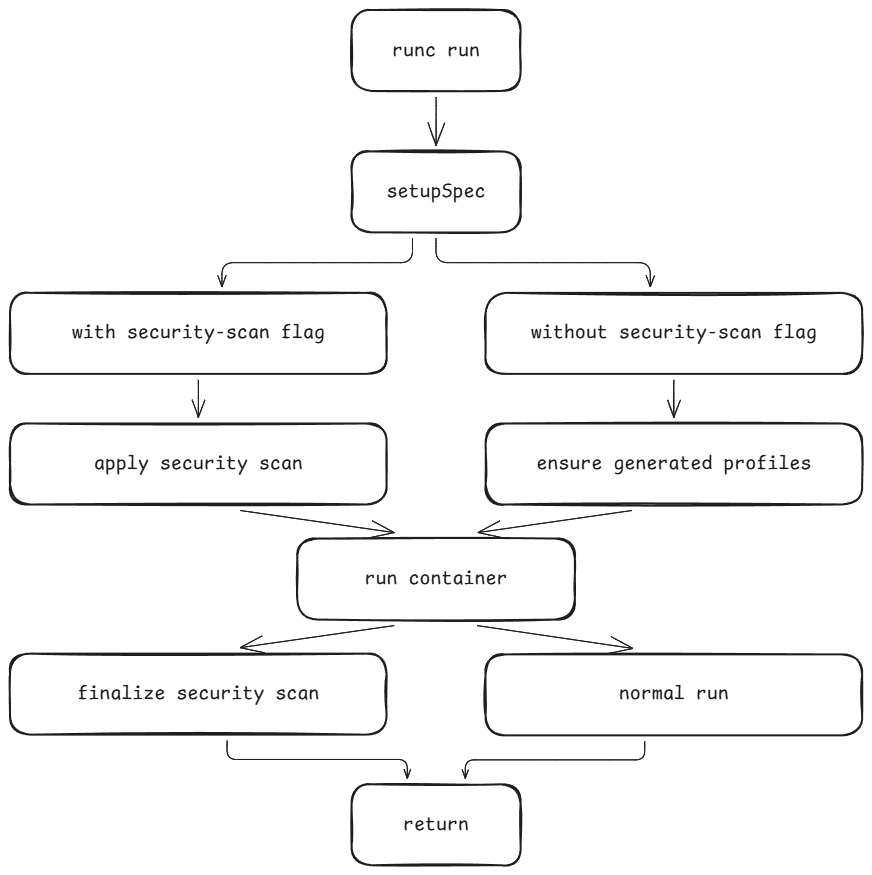
\includegraphics[width=0.82\textwidth]{figs/impl-callflow.png}
\caption{\texttt{runc run} control flow in \texttt{startContainer}. Scan mode generates evidence and finalises it after a successful container run; a normal run only applies previously generated AppArmor state before starting the container.}
\label{fig:impl-callflow}
\end{figure}

\section{Source-Tree Layout}\label{sec:impl-layout}

The fork keeps scanner logic in a small set of Linux-only files. Table~\ref{tab:impl-files} lists the files that are specific to the thesis implementation.

\begin{table}[ht]
\centering
\caption{Implementation files added or modified by the fork.}
\label{tab:impl-files}
\footnotesize
\begin{tabularx}{\textwidth}{>{\raggedright\arraybackslash}p{5.9cm} X}
\toprule
\textbf{File} & \textbf{Responsibility} \\
\midrule
\texttt{src/scanner\_linux.go} & Scanner orchestration: in-memory relaxation, hook installation, tool discovery, AppArmor profile stub generation. \\
\texttt{src/scanner\_hooks\_linux.go} & Hidden self-exec hook sub-commands for AppArmor load/unload, capability snapshot, and capability tracer start/stop. \\
\texttt{src/scanner\_bpf\_linux.go} & cgroup-v2 resolution, bpffs precondition checks, and \texttt{bpftool} map create/update/teardown. \\
\texttt{src/scanner\_apparmor\_linux.go} & AppArmor audit parsing and rule synthesis from \texttt{ALLOWED}/\texttt{DENIED} kernel records. \\
\texttt{src/scanner\_finalize\_linux.go} & One-time spec backup and finalisation of capabilities, seccomp, and AppArmor into \texttt{config.json}. \\
\texttt{src/scanner\_apply\_linux.go} & Auto-load generated AppArmor profiles on later non-scan \texttt{runc run} invocations. \\
\texttt{src/run.go}, \texttt{src/create.go} & CLI flag registration. Only \texttt{run} exposes \texttt{-{}-security-scan}; both expose capability preset flags. \\
\texttt{src/utils\_linux.go} & Capability preset selection, \texttt{startContainer} wiring, and finalisation call site. \\
\texttt{libcontainer/specconv/example.go} & New \texttt{runc spec} template with an empty default capability set. \\
\texttt{tests/integration/}\\\texttt{security\_scan.bats}, \texttt{contrib/runc-}\\\texttt{security-scan-stub-*} & Root-only integration smoke tests and stub tracing tools. \\
\bottomrule
\end{tabularx}
\end{table}

The implementation uses build tags indirectly through file names: scanner files end in \texttt{\_linux.go}, matching the Linux-only nature of seccomp, capabilities, AppArmor, cgroups, and BPF. Non-scan invocations pay only for capability preset resolution and, when a generated AppArmor profile is already referenced by the spec, a best-effort load check.

\section{Capability Defaults}\label{sec:impl-caps}

The first change is independent of scan mode: \texttt{runc spec} now emits an empty capability set. The template in \texttt{libcontainer/specconv/example.go} initialises \texttt{Bounding}, \texttt{Permitted}, and \texttt{Effective} as empty arrays. This gives a new bundle the safest baseline and forces capability grants to be explicit.

Two flags restore compatibility when needed:

\begin{verbatim}
runc run --default-capabilities          <id>   # upstream runc, 3 caps
runc run --default-capabilities-docker   <id>   # Docker-style, 14 caps
runc run                                 <id>   # new default, 0 caps
\end{verbatim}

The flags are mutually exclusive. \texttt{resolveCapabilitiesMode} returns an error if both are set, and \texttt{applyCapabilitiesOverride} writes the selected preset into all five OCI buckets: bounding, effective, permitted, inheritable, and ambient. Writing all buckets avoids an inconsistent state where a capability exists in the bounding set but disappears across \texttt{exec(2)} because it was not also effective or permitted.

\begin{table}[ht]
\centering
\caption{Capability presets implemented by the fork.}
\label{tab:impl-cap-presets}
\begin{tabular}{p{4.0cm}p{10.0cm}}
\toprule
\textbf{Mode} & \textbf{Capability set} \\
\midrule
Default & Empty capability arrays in the generated spec. \\
\texttt{-{}-default-capabilities} & \texttt{CAP\_AUDIT\_WRITE}, \texttt{CAP\_KILL}, \texttt{CAP\_NET\_BIND\_SERVICE}. \\
\texttt{-{}-default-capabilities-docker} & Docker's historical fourteen-capability set, including \texttt{CAP\_CHOWN}, \texttt{CAP\_NET\_RAW}, \texttt{CAP\_SYS\_CHROOT}, and related basic container privileges. \\
\bottomrule
\end{tabular}
\end{table}

\section{Scan Setup and Spec Relaxation}\label{sec:impl-scan-setup}

\texttt{applySecurityScan} begins by resolving the bundle directory and creating \texttt{generated/}. It then resolves the absolute path of the running \texttt{runc} binary with \texttt{os.Executable}; every internal hook uses that binary as \texttt{Hook.Path}. This is the implementation of the self-exec design: the OCI bundle receives hook entries, but no scanner script is written into the bundle.

Before hooks are installed, the in-memory spec is relaxed. \texttt{relaxSpecForScan} clears \texttt{linux.seccomp}, clears \texttt{process.selinuxLabel}, and sets \texttt{process.noNewPrivileges} to \texttt{false}. SELinux is not generated by the thesis fork; clearing the label during scan only prevents an existing label from hiding behaviour that the scanners should observe. \texttt{grantAllCapsForScan} then grants every capability known to the running kernel in all five capability buckets. This broad grant is never persisted: it exists only in the spec passed to the container runner during the recording run.

The scanner logs a warning when the workload runs as \texttt{uid 0}. The kernel skips many \texttt{cap\_capable} checks for root tasks, so a root scan under-reports capability use. The runtime does not rewrite the UID because doing so would break legitimate root workloads; the recommendation is documented as operator guidance instead.

\section{Seccomp Pipeline}\label{sec:impl-seccomp}

Seccomp recording is delegated to \texttt{oci-seccomp-bpf-hook}. The scanner looks for the hook in standard install paths or accepts an explicit \texttt{-{}-scan-seccomp-hook} path. The hook must be executable; otherwise scan mode fails before the container is started.

The scanner writes the OCI annotation
\begin{quote}
\small\path{io.containers.trace-syscall=of:<bundle>/generated/seccomp.json}
\end{quote}
and appends a prestart hook with \texttt{-s}. The generated file is expected to be an OCI \texttt{LinuxSeccomp} object. During finalisation, \texttt{applyGeneratedSeccomp} parses \texttt{generated/seccomp.json} and embeds it into \texttt{spec.Linux.Seccomp}. Empty or malformed seccomp output is treated as a warning and skipped, because the run may have used a CI stub or failed before the external hook wrote a meaningful profile.

The implementation deliberately does not merge with a pre-scan seccomp profile. The scanner cleared that profile in memory so the trace could see the workload's real syscall surface. Re-introducing the original policy by union would make the generated result less tied to observed behaviour.

\section{Capability Tracing Pipeline}\label{sec:impl-cap-trace}

Capability tracing uses BCC's \texttt{capable-bpfcc} with \texttt{-{}-cgroupmap}. A PID-only trace would miss children spawned after the tracer starts; the cgroup map instead matches every task in the container's cgroup. The scanner treats this as a hard requirement and refuses to run when the host cannot satisfy it.

The precondition check in \texttt{requireCapTraceTools} verifies:

\begin{itemize}
    \item \texttt{capable-bpfcc} exists and its help output contains \texttt{-{}-cgroupmap};
    \item \texttt{bpftool} exists;
    \item the host uses the unified cgroup-v2 hierarchy;
    \item \path{/sys/fs/bpf} is mounted as bpffs, except in tests that set \texttt{RUNC\_\allowbreak SCAN\_\allowbreak PIN\_\allowbreak ROOT}.
\end{itemize}

At poststart, \texttt{scan-cap-trace-start} reads the OCI hook state, resolves \path{/proc/<pid>/cgroup} to a cgroup-v2 path, obtains the cgroup id from the directory inode, creates a pinned hash map under \path{/sys/fs/bpf/runc-scan/<id>/cgroup_filter}, inserts the cgroup id, and starts \texttt{capable-bpfcc -{}-cgroupmap <map>}. The tracer PID is written to \texttt{generated/.runc\_cap\_trace.pid}; stdout and stderr go to \texttt{generated/capable-bpfcc.log}.

At poststop, \texttt{scan-cap-trace-stop} sends \texttt{SIGTERM}, waits up to two seconds, escalates to \texttt{SIGKILL} if necessary, deletes the PID file, and removes the pinned map directory. The hook is prepended to the poststop list so the log is closed before finalisation reads it.

\section{AppArmor Pipeline}\label{sec:impl-aa}

AppArmor is generated in two stages. During scan setup, \texttt{buildAppArmorProfileSource} writes a stub profile named \texttt{runc\_scan\_<id>} to \texttt{generated/apparmor.profile}. The profile starts in complain mode with \texttt{attach\_disconnected} and \texttt{mediate\_deleted}, includes \texttt{abstractions/base}, \texttt{abstractions/nameservice}, and \texttt{abstractions/ssl\_certs}, and otherwise stays intentionally small so the audit log reveals what the workload actually touches.

If AppArmor is enabled, a createRuntime hook \texttt{scan-aa-load} loads the profile through \texttt{apparmor\_parser -r} and records the load timestamp in \texttt{generated/.runc\_aa\_started\_at}. A poststop hook \texttt{scan-aa-unload} first collects audit records for that profile and then unloads it with \texttt{apparmor\_parser -R}. Parser failures are logged to \texttt{generated/apparmor-load.log} but are non-fatal, because missing AppArmor userspace tooling should not leave the container teardown path wedged.

The audit collector in \texttt{src/scanner\_apparmor\_linux.go} reads \texttt{journalctl -k} and falls back to \texttt{dmesg}. It filters by profile name and scan time window, and it accepts both \texttt{apparmor=DENIED} and \texttt{apparmor=ALLOWED}. The second form is essential: in complain mode the kernel often logs would-be denials as \texttt{ALLOWED}. File operations are mapped to AppArmor path rules, capability operations to \texttt{capability NAME,} rules, and unsupported operations are preserved as comments. The resulting block is inserted between sentinel markers inside \texttt{apparmor.profile}; rerunning the scan replaces the block rather than appending duplicates.

If the collector wrote at least one rule block, finalisation removes the \texttt{complain} flag from the profile header, turning the file into an enforce-mode profile. If no rules were collected, the profile remains in complain mode. This avoids turning an empty stub into a policy that would deny almost everything on the next run.

\section{Finalisation}\label{sec:impl-final}

\texttt{finalizeSecurityScan} reconciles \texttt{config.json} with the three generated artefact families. It first copies the pre-scan spec to \texttt{generated/spec.original.json}; the backup is created only once so repeated scans do not erase the original rollback target.

The finalisation step then performs three independent rewrites:

\begin{enumerate}
    \item \textbf{Capabilities.} \texttt{generated/capable-bpfcc.log} is parsed for \texttt{CAP\_*} names. The discovered set replaces all five OCI capability buckets. An empty log means an empty set, not the old set.
    \item \textbf{Seccomp.} \texttt{generated/seccomp.json} is parsed as \texttt{LinuxSeccomp} and written into \texttt{linux.seccomp} when it contains a valid \texttt{defaultAction}.
    \item \textbf{AppArmor.} The profile name is parsed from \texttt{generated/apparmor.profile} and written into \texttt{process.apparmorProfile}; if audit rules exist, the profile is flipped out of complain mode.
\end{enumerate}

The updated spec is written through a temporary file and \texttt{rename(2)}, so a crash during finalisation does not leave a half-written \texttt{config.json}. The semantics are replace-from-evidence rather than merge-with-history. This is the main safety invariant of the implementation: a scan cannot grant a capability merely because it used to appear in \texttt{config.json}; only observed capability names survive.

\section{Applying Generated Profiles}\label{sec:impl-apply}

After a successful scan, a later enforcement run is simply a normal \texttt{runc run} on the same bundle. Capabilities and seccomp need no special runtime path because finalisation already embedded them into \texttt{config.json}. AppArmor is different: \texttt{process.apparmorProfile} names a kernel policy, while \texttt{generated/apparmor.profile} is only a text file until loaded.

\texttt{ensureGeneratedProfiles} handles this case for non-scan invocations. It checks that \texttt{process.\allowbreak apparmorProfile} starts with \texttt{runc\_\allowbreak scan\_}, that \path{generated/apparmor.profile} exists, and that the profile name in the file matches the spec. When the check passes and AppArmor is enabled, it calls \texttt{apparmor\_parser -r} before the container starts. Missing parser or disabled AppArmor is logged; if the spec still asks for an unloaded profile, libcontainer will surface the real start error later.

This auto-load path is what makes the one-flag workflow practical: scan once, then rerun the bundle normally. The operator does not need to add a separate AppArmor load command between scan and enforcement.

\section{Generated Bundle Layout}\label{sec:impl-bundle}

A scan writes only data files and hook state under \texttt{generated/}. No executable helper is copied into the bundle.

\begin{verbatim}
<bundle>/generated/
  seccomp.json
  apparmor.profile
  apparmor-README.txt
  apparmor-load.log
  capable-bpfcc.log
  capabilities-from-proc-status.txt
  spec.original.json
  .runc_cap_trace.pid
  .runc_aa_started_at
\end{verbatim}

\texttt{capabilities-from-proc-status.txt} is diagnostic only. It records the kernel-granted \texttt{Cap*} masks from \texttt{/proc/<init>/status}; finalisation relies on \texttt{capable-bpfcc.log}, because granted privileges and used privileges are different facts.

\section{Tests and Current Limits}\label{sec:impl-tests}

The scanner is covered by table-driven unit tests and by a root-only integration smoke test. Unit tests cover capability-name parsing, finalisation behaviour, cgroup path resolution, BPF map wrapper logic, AppArmor profile-name sanitisation, audit parsing, rule insertion, and auto-load decisions. The integration test \texttt{tests/integration/security\_scan.bats} runs \texttt{runc run -{}-security-scan} on a busybox bundle with stubbed \texttt{oci-seccomp-bpf-hook}, \texttt{capable-bpfcc}, and \texttt{bpftool}. It verifies that generated artefacts exist, that \texttt{config.json} receives seccomp and AppArmor state, and that cgroup-wide capability output is aggregated into the narrowed capability set.

The real-kernel evaluation is outside the runtime repository, in the \texttt{runc-hardened-test} laboratory. It uses Ubuntu~24.04, AppArmor, cgroup~v2, real BCC tooling, and the vulnerable Flask workload discussed in Chapter~\ref{ch:experiments}.

Several limitations remain visible in the implementation:

\begin{itemize}
    \item capability tracing under-reports when the workload runs as \texttt{uid 0}; the runtime warns but does not rewrite the UID;
    \item file capabilities, such as \texttt{CAP\_NET\_RAW} carried by \texttt{ping}, are not yet merged from \texttt{security.capability} extended attributes;
    \item cgroup-wide tracing requires cgroup~v2, bpffs, \texttt{bpftool}, and a recent \texttt{capable-bpfcc}; hosts without them are rejected instead of falling back to PID tracing;
    \item AppArmor rule synthesis currently handles common file and capability records and preserves other events as comments for operator review;
    \item profile quality remains bounded by scan coverage, as with any dynamic profiler.
\end{itemize}

These limits do not contradict the design goals; they define the boundary of the prototype evaluated in this thesis and motivate the future work in Chapter~\ref{ch:conclusion}.
